\documentclass[a4paper,11pt,draft]{article}

\usepackage[finnish]{babel}
\usepackage[utf8]{inputenc}
\usepackage[margin=2cm]{geometry}
\usepackage{amsfonts,amsmath,amssymb,amsthm,enumitem}
\usepackage{pgf}
\usepackage{tikz}
\usetikzlibrary{arrows,automata}

\newtheorem*{claim}{Väite}

\newcommand{\set}[1]{{\left\{ #1 \right\}}}
\newcommand{\stateseq}[5]{{%
\begin{automata}[1.3]
      \tikzstyle{every state}=[fill=none,draw=none,text=black,minimum
        size=0.8cm,inner sep=0cm]
      \node[state]                     (r1)                   {$#2_1$};
      \node[state,node distance=#5]    (r2)   [right of=r1]   {$#2_2$};
      \node[state]                     (dots) [right of=r2]   {$\ldots$};
      \node[state]                     (rn)   [right of=dots] {$#2_{n+1}$};
      \node[state,node distance=0.5cm] (sa)   [below of=r1]   {$#3$};
      \node[state,node distance=0.5cm] (dsa)  [below of=r2]   {$#4$};

        \path (r1)   edge [bend left=20] node {$#1_1$} (r2)
              (r2)   edge [bend left] node {$#1_2$} (dots)
              (dots) edge [bend left] node {$#1_n$} (rn);
    \end{automata}%
}}

\newenvironment{automata}[1][2.8]%
{\begin{tikzpicture}[->,>=stealth',shorten >=1pt,auto,node distance=#1cm,semithick]}%
{\end{tikzpicture}}


\begin{document}

\subsection*{582206 Laskennan mallit, syksy 2012\\
2. Harjoitusten malliratkaisut\\
{\rm
\begin{tabular}{ccc}
Jani Rahkola & ja & Juhana Laurinharju
\end{tabular}
}}

\begin{enumerate}
\item
  Olkoon kahden äärellisen automaatin $M_1$ ja $M_2$ tilat ja
  siirtymät seuraavat.
  
  \begin{enumerate}
  \item
    Mikä on kunkin automaatin aloitustila?
  \item
    Mitkä ovat hyväksyviä tiloja?
  \item
    Minkä tilajonon automaatit käyvät läpi syötteellä $aabb$?
  \item
    Hyväksyvätkö automaatit syötteen $aabb$?
  \item
    Hyväksyvätkö automaatit merkkijonon $\varepsilon$?
  \end{enumerate}

  \begin{tabular}{ccc}
  &
    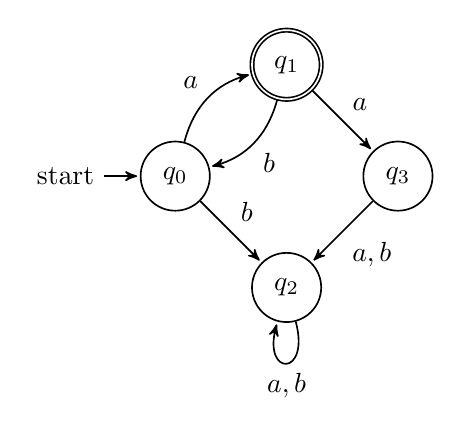
\begin{tikzpicture}[->,>=stealth',shorten >=1pt,auto,node distance=2.0cm,semithick]
      \node[initial,state]   (A)                    {$q_0$};
      \node[accepting,state] (B) [above right of=A] {$q_1$};
      \node[state]           (C) [below right of=A] {$q_2$};
      \node[state]           (D) [below right of=B] {$q_3$};

      \path (A) edge [bend left]  node {$a$} (B)
                edge              node {$b$} (C)
            (B) edge              node {$a$} (D)
                edge [bend left]  node {$b$} (A)
            (C) edge [loop below] node {$a,b$} (C)
            (D) edge              node {$a,b$} (C);
    \end{tikzpicture}
    &
    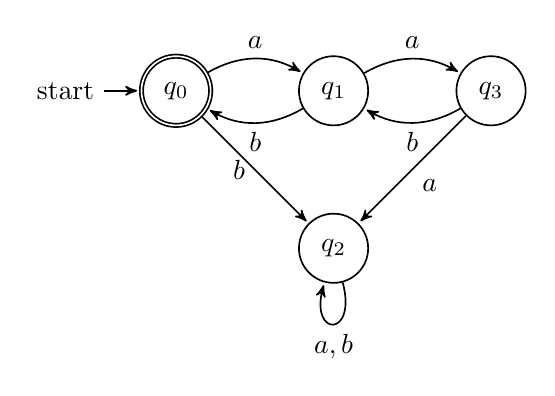
\begin{tikzpicture}[->,>=stealth',shorten >=1pt,auto,node distance=2.0cm,semithick]
      \node[initial,accepting,state]   (A)              {$q_0$};
      \node[state]                     (B) [right of=A] {$q_1$};
      \node[state]                     (C) [below of=B] {$q_2$};
      \node[state]                     (D) [right of=B] {$q_3$};

      \path (A) edge [bend left]   node {$a$}        (B)
                edge               node [left] {$b$} (C)
            (B) edge [bend left]   node {$a$}        (D)
                edge [bend left]   node {$b$}        (A)
            (C) edge [loop below]  node {$a,b$}      (C)
            (D) edge               node {$a$}        (C)
                edge [bend left]   node {$b$}        (B);
    \end{tikzpicture}
    \\
        & $M_1$             & $M_2$ \\
    (a) & $q_0$             & $q_0$ \\
    (b) & $\set{q_1}$       & $\set{q_0}$ \\
    (c) & $q_0q_1q_3q_2q_2$ & $q_0q_1q_3q_1q_0$ \\
    (d) & ei                & kyllä \\
    (e) & ei                & kyllä


\end{tabular}
\item Olkoon äärellisen automaatin $M$ formaali kuvaus
  $(\set{q_1,q_2,q_3,q_4,q_5}, \set{u,d}, \delta, q_3, \set{q_3})$ missä
  siirtymäfunktion määrittelee taulukko:
\[
\begin{array}{c|cc}
    & u   & d   \\ \hline
q_1 & q_1 & q_2 \\
q_2 & q_1 & q_3 \\
q_3 & q_2 & q_4 \\
q_4 & q_3 & q_5 \\
q_5 & q_4 & q_5
 \end{array} 
\]
Piirrä automaatti $M$ (tilat ja siirtymät).

\begin{automata}
  \node[state]                   (q1)               {$q_1$};
  \node[state]                   (q2)  [left of=q1] {$q_2$};
  \node[state,initial above,accepting] (q3)  [left of=q2] {$q_3$};
  \node[state]                   (q4)  [left of=q3] {$q_4$};
  \node[state]                   (q5)  [left of=q4] {$q_5$};


  \path (q1) edge [loop right] node {$u$} (q1)
             edge [bend right] node {$d$} (q2)
        (q2) edge [bend right] node {$u$} (q1)
             edge [bend right] node {$d$} (q3)
        (q3) edge [bend right] node {$u$} (q2)
             edge [bend right] node {$d$} (q4)
        (q4) edge [bend right] node {$u$} (q3)
             edge [bend right] node {$d$} (q5)
        (q5) edge [bend right] node {$u$} (q4)
             edge [loop left]  node {$d$} (q5);

\end{automata}

\newpage

\item Minkälaisia merkkijonoja eli sanoja seuraavat äärelliset automaatit hyväksyvät?

\begin{tabular}{cccc}
(a) & 
\begin{tabular}{c}
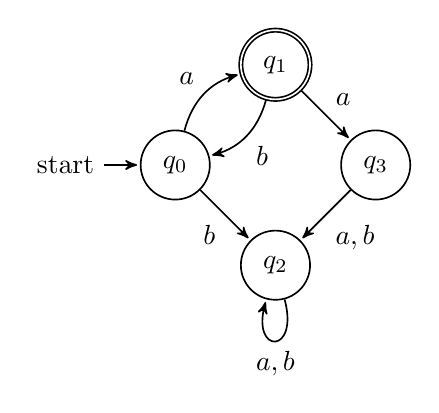
\begin{tikzpicture}[->,>=stealth',shorten >=1pt,auto,node distance=1.8cm,semithick]
 %\tikzstyle{every state}=[fill=red,draw=none,text=white]

 \node[initial,state]  (q0)                     {$q_0$};
 \node[state,accepting](q1) [above right of=q0] {$q_1$};
 \node[state]          (q2) [below right of=q0] {$q_2$};
 \node[state]          (q3) [above right of=q2] {$q_3$};

 \path (q0) edge [bend left]  node       {$a$} (q1)
            edge              node [swap]{$b$} (q2)
       (q1) edge              node       {$a$} (q3)
            edge [bend left] node        {$b$} (q0)
       (q2) edge [loop below] node {$a,b$} ()
       (q3) edge             node {$a,b$} (q2);
\end{tikzpicture} 
\end{tabular}
& (b) &
\begin{tabular}{c}
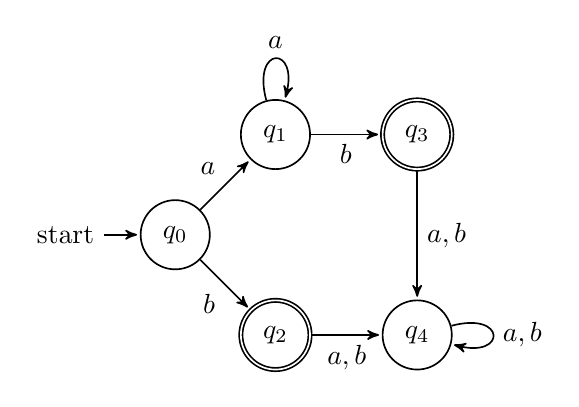
\begin{tikzpicture}[->,>=stealth',shorten >=1pt,auto,node distance=1.8cm,semithick]
 %\tikzstyle{every state}=[fill=red,draw=none,text=white]

 \node[initial,state]   (q0)                     {$q_0$};
 \node[state]           (q1) [above right of=q0] {$q_1$};
 \node[state,accepting] (q2) [below right of=q0] {$q_2$};
 \node[state,accepting] (q3) [right of=q1]       {$q_3$};
 \node[state]           (q4) [right of=q2]       {$q_4$};

 \path (q0) edge              node       {$a$}   (q1)
            edge              node [swap]{$b$}   (q2)
       (q1) edge [loop above] node       {$a$}   ()
            edge              node [swap]{$b$}   (q3)
       (q2) edge              node [swap]{$a,b$} (q4)
       (q3) edge              node       {$a,b$} (q4)
       (q4) edge [loop right] node       {$a,b$} ();    
\end{tikzpicture}
\end{tabular}
\end{tabular}

\begin{tabular}{cccc}
(c) &
\begin{tabular}{c}
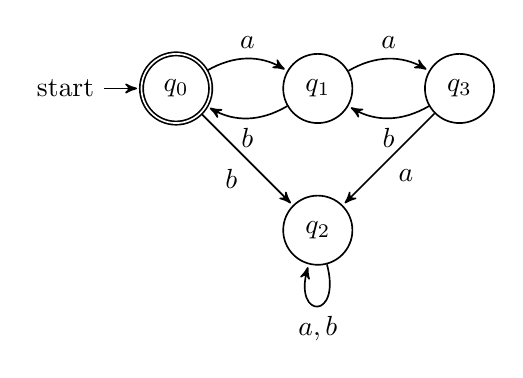
\begin{tikzpicture}[->,>=stealth',shorten >=1pt,auto,node distance=1.8cm,semithick]
 %\tikzstyle{every state}=[fill=red,draw=none,text=white]

 \node[initial,state,accepting]
              (q0)               {$q_0$};
 \node[state]           (q1) [right of=q0] {$q_1$};
 \node[state] (q2) [below of=q1] {$q_2$};
 \node[state] (q3) [right of=q1] {$q_3$};

 \path (q0) edge [bend left]  node       {$a$}   (q1)
            edge              node [swap]{$b$}   (q2)
       (q1) edge [bend left]  node       {$a$}  (q3)
            edge [bend left]  node       {$b$}   (q0)
       (q2) edge [loop below] node       {$a,b$} ()
       (q3) edge              node       {$a$}   (q2)
       (q3) edge [bend left]  node       {$b$} (q1);
\end{tikzpicture}
\end{tabular}
& (d) &
\begin{tabular}{c}
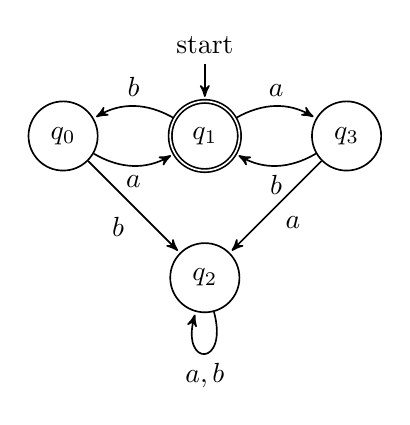
\begin{tikzpicture}[->,>=stealth',shorten >=1pt,auto,node distance=1.8cm,semithick]
 %\tikzstyle{every state}=[fill=red,draw=none,text=white]

 \node[state] (q0)               {$q_0$};
 \node[state,initial above,accepting]
              (q1) [right of=q0] {$q_1$};
 \node[state] (q2) [below of=q1] {$q_2$};
 \node[state] (q3) [right of=q1] {$q_3$};

 \path (q0) edge [bend right]  node [swap]{$a$}   (q1)
            edge              node [swap]{$b$}   (q2)
       (q1) edge [bend left]  node       {$a$}  (q3)
            edge [bend right]  node [swap]{$b$}   (q0)
       (q2) edge [loop below] node       {$a,b$} ()
       (q3) edge              node       {$a$}   (q2)
       (q3) edge [bend left]  node       {$b$} (q1);
\end{tikzpicture}
\end{tabular}
\end{tabular}

\begin{tabular}{cccc}
(e) &
\begin{tabular}{c}
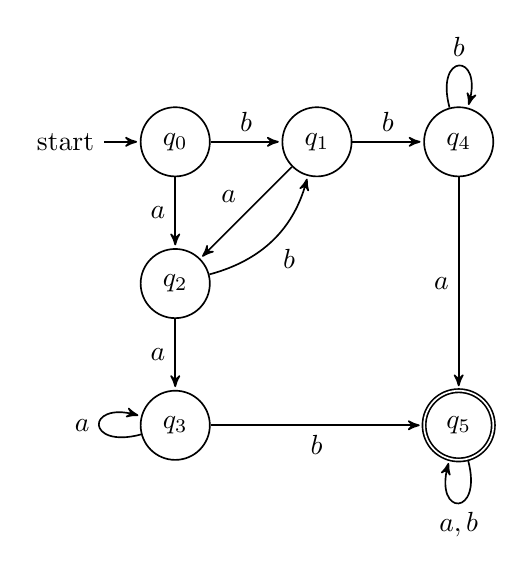
\begin{tikzpicture}[->,>=stealth',shorten >=1pt,auto,node distance=1.8cm,semithick]
 %\tikzstyle{every state}=[fill=red,draw=none,text=white]

 \node[state,initial] (q0)               {$q_0$};
 \node[state]       (q1) [right of=q0] {$q_1$};
 \node[state]       (q2) [below of=q0] {$q_2$};
 \node[state]       (q3) [below of=q2] {$q_3$};
 \node[state]       (q4) [right of=q1]  {$q_4$};
 \node              (qx)[below of=q4] {};
 \node[state,accepting](q5)[below of=qx] {$q_5$};
 
 \path (q0) edge              node [swap] {$a$}   (q2)
            edge              node        {$b$}   (q1)
       (q1) edge              node [swap] {$a$}   (q2)
            edge              node        {$b$}   (q4)
       (q2) edge              node [swap] {$a$}   (q3)
            edge [bend right] node [swap] {$b$}   (q1)
       (q3) edge [loop left]  node        {$a$}   (  )
       (q3) edge              node [swap] {$b$}   (q5)
       (q4) edge              node [swap] {$a$}   (q5)
       (q4) edge [loop above] node        {$b$}   (  )
       (q5) edge [loop below] node        {$a,b$} (  );
\end{tikzpicture}
\end{tabular}
\end{tabular}

\begin{enumerate}
  \item $a,aba,ababa,abababa,\ldots = \set{a} \circ \set{ba}^* = a(ba)^*$
  \item Merkkijonot joiden alussa on mielivaltainen määrä $a$-merkkiä ja
    lopuksi yksi $b$.
    %
    \begin{equation*}
      \set{a}^* \circ \set{b} = a^*b
    \end{equation*}

  \item Sisältää saman määrän $a$:ta ja $b$:tä eikä missään kohdassa ei ole
    ollut siihen mennessä enempää $b$:tä kuin $a$:ta eikä missään kohdassa
    ole ollut siihen mennessä kolmea $a$:ta enem\-män kuin $b$:tä.
%
    \begin{equation*}
      (\set{a} \circ \set{ab}^* \circ \set{b})^* = (a(ab)^*b)^*
    \end{equation*}

  \item Muodostettu laittamalla merkkijonoja $ab$ ja $ba$ peräkkäin
    mielivaltaisesti.
%
    \begin{equation*}
      \set{ab,ba}^* = (ab|ba)^*
    \end{equation*}

  \item Sisältää merkkijonon $aab$ tai $bba$.

  \begin{equation*}
    \set{a,b}^* \circ \set{aab,bba} \circ \set{a,b}^* =
    (a|b)^*(aab|bba)(a|b)^*
  \end{equation*}
\end{enumerate}

\item Piirrä äärelliset automaatit tiloineen ja siirtymänuolineen seuraaville kielille.
\begin{enumerate}
\item $L = \set{w \in \set{a, b}^* \mid \mbox{$w$ sisältää ainakin yhden $a$:n}}$

    \begin{center}
    \begin{automata}
        \node[initial,state]   (q1)               {$q_1$};
        \node[accepting,state] (q2) [right of=q1] {$q_2$};

        \path (q1) edge [loop above] node {$b$}   (  )
                   edge              node {$a$}   (q2)
              (q2) edge [loop above] node {$a,b$} (  );
    \end{automata}
    \end{center}

\item $L = \set{w \in \set{a, b}^* \mid \mbox{$w$ alkaa $b$ tai $ab$:llä}}$

    \begin{center}
    \begin{automata}[2]
        \node[initial,state]   (q1)                     {$q_1$};
        \node[state]           (q2) [above right of=q1] {$q_2$};
        \node[accepting,state] (q3) [below right of=q2] {$q_3$};
        \node[state]           (q4) [above of=q2]       {$q_4$};
        
        \path (q1) edge              node {$a$} (q2)
                   edge              node {$b$} (q3)
              (q2) edge              node {$b$} (q3)
                   edge              node {$a$} (q4)
              (q3) edge [loop right] node {$a,b$} ()
              (q4) edge [loop above] node {$a,b$} ();
    \end{automata}
    \end{center}

\item $L = \set{w \in \set{a,b}^*  \mid \mbox{$w$ loppuu $aa$:han}}$

    Suunnitellun automaatin olisi tarkoitus "muistaa", ollaanko nähty nolla,
    yksi vai ainakin kaksi $a$-merkkiä. Luodaan siis automaatille tilat
    jokaista kolmea vaihtoehtoa varten. Alkutilassa ei olla vielä nähty yhtään
    $a$:ta. Tilassa $q_a$ ollaan nähty yksi $a$ ja tilassa $q_{aa}$ ollaan
    nähty ainakin kaksi $a$:ta.

    \begin{center}
    \begin{automata}
        \node[initial,state]   (qe)                {$q_\varepsilon$};
        \node[state]           (qa)  [below of=qe] {$q_a$};
        \node[accepting,state] (qaa) [right of=qa] {$q_{aa}$};

        \path (qe)  edge [loop above] node        {$b$} (  )
                    edge [bend left]  node        {$a$} (qa)
              (qa)  edge [bend left]  node        {$b$} (qe)
                    edge              node        {$a$} (qaa)
              (qaa) edge [loop right] node        {$a$} (  )
                    edge              node [swap] {$b$} (qe);
    \end{automata}
    \end{center}

\item
  $L = \set{w \in \set{a,b}^* \mid \mbox{$w$ sisältää merkkijonon
    $abab$ }}$

  \begin{center}
  \begin{automata}
    \node[initial,state]   (qe)                    {$q_\varepsilon$};
    \node[state]           (qa)    [right of=qe]   {$q_a$};
    \node[state]           (qab)   [right of=qa]   {$q_{ab}$};
    \node[state]           (qaba)  [right of=qab]  {$q_{aba}$};
    \node[accepting,state] (qabab) [right of=qaba] {$q_{abab}$};

    \path (qe)    edge [loop above] node        {$b$}   ()   
                  edge              node        {$a$}   (qa)   
          (qa)    edge [loop below] node        {$a$}   ()     
                  edge              node        {$b$}   (qab)  
          (qab)   edge [bend right] node [swap] {$b$}   (qe)   
                  edge              node        {$a$}   (qaba) 
          (qaba)  edge [bend left]  node        {$a$}   (qa)       
                  edge              node        {$b$}   (qabab)
          (qabab) edge [loop above] node        {$a,b$} ();
  \end{automata}
  \end{center}

\item
  $L = \set{w \in \set{a,b}^* \mid \mbox{jokaisen $w$:ssä olevan $a$:n
    edessa on $b$}}$
  
  \begin{center}
  \begin{automata}
    \node[initial,accepting,state] (q1)                     {$q_1$};
    \node[accepting,state]         (q2) [above right of=q1] {$q_2$};
    \node[state]                   (q3) [below right of=q1] {$q_3$};

    \path (q1) edge              node        {$a$}   (q3)
               edge [bend right] node [swap] {$b$}   (q2)
          (q2) edge [bend right] node [swap] {$a$}   (q1)
               edge [loop right] node        {$b$}   ()
          (q3) edge [loop right] node        {$a,b$} ();
  \end{automata}
  \end{center}

\end{enumerate}

\newpage

\item
  Olkoon kielet $A$ ja $B$ säännöllisiä. Todista että joukkoerotus $A
  - B$ tuottaa säännöllisen kielen luentokalvojen yhdisteen esimerkin
  mukaisesti. Piirrä myös pieni esimerkki automaateista $L(M_1)=A$,
  $L(M_2)= B$ ja $L(M_{A-b})=A-B$.

  Koska $A$ ja $B$ ovat säännöllisiä, on olemassa äärelliset
  automaatit $M_A = (Q_A, \Sigma, \delta_A, s_A, F_A)$ ja $M_B = (Q_B,
  \Sigma, \delta_B, s_B, F_B)$ jotka tunnistavat kielet $A$ ja $B$.
  Siis $L(M_A) = A$ ja $L(M_B) = B$.

  Määritellään automaatti $M_{A-B} = (Q_{A-B}, \Sigma, \delta_{A-B},
  s_{A-B}, F_{A-B})$ missä
%
  \begin{align*}
    Q_{A-B} &= Q_A \times Q_B \\
    \delta_{A-B}((q_A, q_B), a) &= (\delta_A(q_A,a), \delta_B(q_B,a)) \\
    s_{A-B} &= (s_A, s_B) \\
    F_{A-B} &= \set{(q_A, q_B) \in Q_{A-B} \mid q_A \in F_A \text{ ja
      } q_B \notin F_B} = F_A \times (Q_B - F_B)
  \end{align*}
%

  Konstruktio on hyvin samanlainen kuin yhdisteautomaatillakin. Automaatti
  simuloi samanaikaisesti molempia alkuperäisiä automaatteja, joten
  tilajoukkona on $Q_A \times Q_B$ joka siis sisältää kaikki parit $(q_A,
  q_B)$, missä $q_A$ on ensimmäisen automaatin tila ja $q_B$ toisen
  automaatin tila.

  Tilasiirtymä pitää nyt määritellä pareilta pareille. Määritellään se niin,
  että parin ensimmäisessä tilassa siirrytään ensimmäisen automaatin
  tilasiirtymäfunktiota noudattaen ja toisessa tilassa toisen automaatin
  tilasiirtymäfunktiota noudattaen.

  Hyväksyviä tiloja ovat nyt sellaiset tilaparit $(q_A, q_B)$ joissa
  ensimmäisen automaatin tila $q_A$ on ensimmäisen automaatin hyväksyvä ja
  toinen tila $q_B$ ei ole toisen automaatin hyväksyvä tila.

%
  \begin{claim}
    Yllä määritelty automaatti $M_{A-B}$ tunnistaa kielen $A - B$.
    Siten kieli $A - B$\\ on säännöllinen.
  \end{claim}
%
  \begin{proof}
    Olkoon $w \in \Sigma^*$. Nyt $w = w_1 \ldots w_n$. Määritellään tilajonot
%
    \begin{align*}
      r &= r_1 \ldots r_{n+1} \text{ ja } \\
      p &= p_1 \ldots p_{n+1}
    \end{align*}
%
    joiden läpi automaatit $M_A$ ja $M_B$ kulkevat merkkijonon $w$
    aikana siten, että
%
    \begin{align*}
      r_1     &= s_A              & p_1    &= s_B \\
      r_{i+1} &= \delta_A(r_i,w_i) & p_{i+1} &= \delta_B(p_i, w_i).
    \end{align*}
%
    \begin{center}
      \stateseq{w}{r}{s_A}{\delta_A(s_A,w_1)}{1.7cm}
      \stateseq{w}{p}{s_B}{\delta_B(s_B,w_1)}{1.7cm}
    \end{center}
%
    Automaatti $M_A$ kulkee syötteellä $w$ tilajonon $r$ ja automaatti
    $M_B$ tilajonon $p$ läpi. Siis esimerkiksi automaatti $M_A$
    siirtyy merkillä $w_i$ tilasta $r_i$ tilaan $r_{i+1}$.

    Määritellään myös vastaavasti jono
% 
   \begin{equation*}
      q = q_{1} \ldots q_{n+1}
    \end{equation*}
% 
   jonka läpi automaatti $M_{A-B}$ kulkee syötteellä $w$. Nyt siis
%
    \begin{align*}
      q_1 &= s_{A-B} = (s_A, s_B) = (r_1,p_1) \\
      q_{i+1} &= \delta_{A-B}(q_i, w_i).
    \end{align*}
%
    \begin{center}
      \stateseq{w}{q}{s_{A-B}}{\delta_{A-B}(s_{A-B},w_1)}{2.5cm}
    \end{center}
%
    Intuitiivisesti näyttäisi siltä, että $q_i = (r_i,p_i)$, sillä
%
    \begin{align*}
      q_1 &= (r_1, p_1) \\
      q_2 &= \delta_{A-B}(q_1, w_1) \\
          &= (\delta_A(r_1, w_1), \delta_B(p_1, w_1) \\
          &= (r_2, p_2) \\
      \ldots &
    \end{align*}
%
    Näytetään tämä todeksi induktiolla.
%
    \begin{claim}
      $q_i = (r_i,p_i)$ tai $n+1 < i$
    \end{claim}
%
    \begin{proof}
      \begin{description} \item[]
        \item[Alkuaskel] Määritelmän nojalla $q_1 = (r_1,p_1)$.
        \item[Induktioaskel]
          \begin{description}\item[]
            \item[Induktio-oletus] $i > n+1$ tai $q_i = (r_i,p_i)$
            \item[Induktioaskeleen väite] $i+1 > n+1$ tai $q_{i+1} =
            (r_{i+1}, p_{i+1})$

            \item[Induktioaskeleen todistus] \mbox{} %tyhjä kappale

            Jos $i \ge n+1$, niin $i+1 > n+1$. Tarkastellaan siis tapausta
            $i < n+1$. Nyt
%
            \begin{align*}
              q_{i+1} &= \delta_{A-B}(q_i, w_i)
                         &\text{$q_{i+1}$:n määritelmä}\\
                      &= \delta_{A-B}((r_i, p_i), w_i)
                         &\text{induktio-oletus} \\
                      &= (\delta_A(r_i, w_i), \delta_B(p_i, w_i))
                         &\text{$\delta_{A-B}$:n määritelmä}\\
                      &= (r_{i+1}, p_{i+1})
                         &\text{$r_{i+1}$:n ja $p_{i+1}$:n määritelmät.}
            \end{align*}
          \end{description}
      \end{description}
    \end{proof}
%

    Automaatti $M_{A-B}$ hyväksyy merkkijonon $w$ jos ja vain jos
    $q_{n+1} \in F_{A-B}$. Näytetään nyt, että $M_{A-B}$ hyväksyy merkkijonon
    $w$ täsmälleen silloin kun $w$ kuuluu kieleen $A -B$.
%
    \begin{align*}
      q_{n+1} \in F_{A-B}
      &\Leftrightarrow (r_{n+1}, p_{n+1}) \in F_{A-B}
        & \text{ äskeinen induktio}\\
      &\Leftrightarrow r_{n+1} \in F_A \text{ ja } p_{n+1} \notin F_B
        & F_{A-B} \text{:n määritelmä}\\
      &\Leftrightarrow w \in A \text{ ja } w \notin B
        & F_A \text{ tunnistaa kielen $A$ ja $F_B$ $B$:n} \\
      &\Leftrightarrow w \in A - B
        & \text{ joukkoerotuksen $A-B$ määritelmä.}
    \end{align*}
%
    Siis kieli $A - B$ on säännöllinen.
  \end{proof}

\item
  Seuraavat kielet koostettu yksinkertaisemmista kielistä
  säännöllisillä operaatioilla (kaikkia ei vielä todistettu tunnilla).
  Piirrä jokaisessa kohdassa ensin yksinkertaiset kielet tunnistavat
  automaatit tiloineen ja siirtymineen ja piirrä sen perusteella
  lopullinen automaatti (vrt. luentokalvojen yhdisteautomaatti).
  Kaikissa kohdissa $\Sigma = \set{a,b}$.
  \begin{enumerate}
  \item 
    $\set{w \mid \mbox{$w$ sisältää ainakin kolme $a$:ta ja ainakin
      kaksi $b$:tä}}$

    Automaatti joka tunnistaa kielen, jossa jokainen merkkijono
    sisältää ainakin kolme $a$:ta.

    \begin{center}
    \begin{automata}[1.7]
      \node[initial,state]   (qe)                  {$q_{\varepsilon}$};
      \node[state]           (qa)   [right of=qe]  {$q_{a}$};
      \node[state]           (qaa)  [right of=qa]  {$q_{aa}$};
      \node[accepting,state] (qaaa) [right of=qaa] {$q_{aaa}$};

      \path (qe)   edge              node {$a$}   (qa) 
                   edge [loop above] node {$b$}   ()
            (qa)   edge              node {$a$}   (qaa)
                   edge [loop above] node {$b$}   ()
            (qaa)  edge              node {$a$}   (qaaa)
                   edge [loop above] node {$b$}   ()
            (qaaa) edge [loop above] node {$a,b$} ();
    \end{automata}
    \end{center}

    Lisäksi toinen automaatti joka tunnistaa kielen, jossa jokainen
    merkkijono sisältää ainakin kaksi $b$:tä.

    \begin{center}
    \begin{automata}[1.7]
      \node[initial,state]   (qe)                  {$q_{\varepsilon}$};
      \node[state]           (qb)   [right of=qe]  {$q_{b}$};
      \node[accepting,state] (qbb)  [right of=qb]  {$q_{bb}$};

      \path (qe)  edge              node {$b$}   (qb) 
                  edge [loop above] node {$a$}   ()
            (qb)  edge              node {$b$}   (qbb)
                  edge [loop above] node {$a$}   ()
            (qbb) edge [loop above] node {$a,b$} ();
    \end{automata}
    \end{center}

    Muodostetaan näistä automaateista leikkausautomaatti. Automaatti
    pitää samanaikaisesti kirjaa siitä, missä tilassa kumpikin
    automaatti tällä hetkellä menee ja hyväksyy silloin, kun kumpikin
    alkuperäisistä automaateista hyväksyy.

    Leikkausautomaatin tilat ovat nyt siis jälleen pareja, mutta nyt
    hyväksyviä tiloja ovat vain sellaiset parit $(q_a, q_b)$ missä
    $q_a$ on ensimmäisen automaatin hyväksyvä tila ja $q_b$ on toisen
    automaatin hyväksyvä tila.

    Tilannetta voi havainnollistaa piirtämällä toisen alkuperäisistä automaateista
    vaakasuunnassa ja toisen pystysuunnassa. Leikkausautomaatin voi
    piirtää nyt hilaksi näiden viereen.

    \begin{automata}[2.6]

      \node[initial above,state]   (qee)                 {$(q_\varepsilon, q_\varepsilon)$};
      \node[state]           (qae)     [right of=qee]     {$(q_\varepsilon, q_a)$};
      \node[state]           (qaae)    [right of=qae] {$(q_\varepsilon, q_{aa})$};
      \node[state]           (qaaae)   [right of=qaae] {$(q_\varepsilon, q_{aaa})$};
      \node[state]           (qeb)     [below of=qee]     {$(q_b, q_\varepsilon)$};
      \node[state]           (qab)    [right of=qeb]    {$(q_b, q_a)$};
      \node[state]           (qaab)   [right of=qab]   {$(q_b, q_{aa})$};
      \node[state]           (qaaab)  [right of=qaab]  {$(q_b, q_{aaa})$};
      \node[state]           (qebb)    [below of=qeb]    {$(q_{bb}, q_\varepsilon)$};
      \node[state]           (qabb)   [right of=qebb]   {$(q_{bb}, q_a)$};
      \node[state]           (qaabb)  [right of=qabb]  {$(q_{bb}, q_{aa})$};
      \node[accepting,state] (qaaabb) [right of=qaabb] {$(q_{bb}, q_{aaa})$};

      \path (qee) edge node {$a$} (qae)
            (qae) edge node {$a$} (qaae)
            (qaae) edge node {$a$} (qaaae)
            (qeb) edge node {$a$} (qab)
            (qab) edge node {$a$} (qaab)
            (qaab) edge node {$a$} (qaaab)
            (qebb) edge node {$a$} (qabb)
            (qabb) edge node {$a$} (qaabb)
            (qaabb) edge node {$a$} (qaaabb)
            (qee) edge node {$b$} (qeb)
            (qeb) edge node {$b$} (qebb)
            (qae) edge node {$b$} (qab)
            (qab) edge node {$b$} (qabb)
            (qaae) edge node {$b$} (qaab)
            (qaab) edge node {$b$} (qaabb)
            (qaaae) edge node {$b$} (qaaab)
            (qaaab) edge node {$b$} (qaaabb)

            (qebb) edge [loop below] node {$b$} ()
            (qabb) edge [loop below] node {$b$} ()
            (qaabb) edge [loop below] node {$b$} ()
            (qaaae) edge [loop right] node {$a$} ()
            (qaaab) edge [loop right] node {$a$} ()
            (qaaabb) edge [out=330, in=300,looseness=8] node {$a,b$} (qaaabb);


      \node[initial above,state, node distance=2cm]   (qeb)  [left of=qee] {$q_{\varepsilon}$};
      \node[state]           (qb)   [below of=qeb] {$q_{b}$};
      \node[accepting,state] (qbb)  [below of=qb] {$q_{bb}$};

      \path (qeb) edge              node {$b$}   (qb) 
                  edge [loop left] node {$a$}   ()
            (qb)  edge              node {$b$}   (qbb)
                  edge [loop left] node {$a$}   ()
            (qbb) edge [loop left] node {$a,b$} ();


      \node[initial,state]   (qea)  [above of=qee] {$q_{\varepsilon}$};
      \node[state]           (qa)   [right of=qea]  {$q_{a}$};
      \node[state]           (qaa)  [right of=qa]  {$q_{aa}$};
      \node[accepting,state] (qaaa) [right of=qaa] {$q_{aaa}$};

      \path (qea)  edge              node {$a$}   (qa) 
                   edge [loop above] node {$b$}   ()
            (qa)   edge              node {$a$}   (qaa)
                   edge [loop above] node {$b$}   ()
            (qaa)  edge              node {$a$}   (qaaa)
                   edge [loop above] node {$b$}   ()
            (qaaa) edge [loop above] node {$a,b$} ();


    \end{automata}

  \item
    $\set{w \mid \mbox{$w$:n pituus on parillinen sisältäen parittoman määrän $a$:ta} }$

    \begin{center}
    \begin{automata}
      \node[initial above, state] (q00a) {$(q_{0}, q_{0a})$};
      \node[accepting,state] (q01a)[below of=q00a]{$(q_{0}, q_{1a})$};
      \node[state] (q10a)[right of=q00a]{$(q_{1}, q_{0a})$};
      \node[state] (q11a)[right of=q01a]{$(q_{1}, q_{1a})$};

      \path (q00a) edge [bend left=15] node {$a$} (q11a)
            (q00a) edge  node {$b$} (q10a)
            (q01a) edge [bend left=15] node {$a$} (q10a)
            (q01a) edge [bend right=40] node [swap] {$b$} (q11a)
            (q10a) edge [bend left=15] node {$a$} (q01a)
            (q10a) edge [bend right=40] node [swap] {$b$} (q00a)
            (q11a) edge [bend left=15] node {$a$} (q00a)
            (q11a) edge  node {$b$} (q01a) ;

      \node[state, initial, accepting] (q0) [above of=q00a] {$q_{0}$};
      \node[state]          (q1) [right of=q0]   {$q_{1}$};


      \path (q0) edge [bend left] node {$a,b$} (q1)
            (q1) edge [bend left] node {$a,b$} (q0) ;

      \node[state, initial above, node distance=2cm] (q0a) [left of=q00a] {$q_{0a}$};
      \node[state, accepting]          (q1a) [below of=q0a] {$q_{1a}$};


      \path (q0a) edge [loop left] node {$b$} (q0a)
            (q1a) edge [loop left] node {$b$} (q1a)
            (q0a) edge [bend left] node {$a$} (q1a)
            (q1a) edge [bend left] node {$a$} (q0a) ;

    \end{automata}
    \end{center}

  \item
    $\set{w \mid \mbox{$w$:ssä olevin $a$-merkkien määrä ei ole kaksi} }$

    Tehdään ensin automaatti, joka hyväksyy vain merkkijonot joissa on tasan
    kaksi $a$:ta.

    \begin{automata}
      \node[state, initial]   (q0a)                {$q_{0a}$};
      \node[state]            (q1a) [right of=q0a] {$q_{1a}$};
      \node[state, accepting] (q2a) [right of=q1a] {$q_{2a}$};
      \node[state]            (q3a) [right of=q2a] {$q_{3a}$};


      \path (q0a) edge [loop above] node {$b$} (q0a)
            (q1a) edge [loop above] node {$b$} (q1a)
            (q2a) edge [loop above] node {$b$} (q2a)
            (q3a) edge [loop above] node {$b$} (q3a)
            (q0a) edge              node {$a$} (q1a)
            (q1a) edge              node {$a$} (q2a)
            (q2a) edge              node {$a$} (q3a)
            (q3a) edge [loop above] node {$a$} (q3a) ;

    \end{automata}

    Nyt tästä saadaan merkkijono joka hyväksyy kaikki merkkijonot joissa ei
    ole tasan kahta $a$-merkkiä vaihtamalla hyväksyvät ja hylkäävät tilat
    keskenään.

    \begin{automata}
      \node[state, initial, accepting]   (q0a)                {$q_{0a}$};
      \node[state, accepting]            (q1a) [right of=q0a] {$q_{1a}$};
      \node[state] (q2a) [right of=q1a] {$q_{2a}$};
      \node[state, accepting]            (q3a) [right of=q2a] {$q_{3a}$};


      \path (q0a) edge [loop above] node {$b$} (q0a)
            (q1a) edge [loop above] node {$b$} (q1a)
            (q2a) edge [loop above] node {$b$} (q2a)
            (q3a) edge [loop above] node {$b$} (q3a)
            (q0a) edge              node {$a$} (q1a)
            (q1a) edge              node {$a$} (q2a)
            (q2a) edge              node {$a$} (q3a)
            (q3a) edge [loop above] node {$a$} (q3a) ;

    \end{automata}

  \item
    $\set{w \mid \mbox{$w$ ei sisällä alimerkkijonoja $ab$ ja $ba$} }$

    Muodostetaan ensin automaatti joka tunnistaa merkkijonon, joka sisältää
    sekä merkkijonon $ab$ että $ba$. Tehdään tämä kuten aikaisemmissakin
    kohdissa.

    \begin{center}
    \begin{automata}
      \node[state,initial above] (qe_e)     {$(q_{e}, q_{e})$};
      \node[state] (qe_b)  [below of=qe_e]  {$(q_{e}, q_{b})$};
      \node[state] (qe_ba) [below of=qe_b]  {$(q_{e}, q_{ba})$};
      \node[state] (qa_e)  [right of=qe_e]  {$(q_{a}, q_{e})$};
      \node[state] (qab_e) [right of=qa_e]  {$(q_{ab}, q_{e})$};
      \node[state] (qa_b)  [right of=qe_b]  {$(q_{a}, q_{b})$};
      \node[state] (qab_b) [right of=qa_b]  {$(q_{ab}, q_{b})$};
      \node[state] (qa_ba) [right of=qe_ba] {$(q_{a}, q_{ba})$};
      \node[accepting,state] (qab_ba)[right of=qa_ba] {$(q_{ab}, q_{ba})$};

      \path (qe_e)   edge              node {$a$} (qa_e)
            (qe_b)   edge              node {$a$} (qa_ba)
            (qe_ba)  edge              node {$a$} (qa_ba)
            (qe_e)   edge              node {$b$} (qe_b)
            (qe_b)   edge [in=20, out=50, looseness=8] node {$b$} (qe_b)
            (qe_ba)  edge [loop below] node {$b$} (qe_ba)
            (qa_e)   edge [loop above] node {$a$} (qa_e)
            (qa_b)   edge              node {$a$} (qa_ba)
            (qa_ba)  edge [loop below] node {$a$} (qa_ba)
            (qa_e)   edge              node {$b$} (qab_b)
            (qa_b)   edge              node {$b$} (qab_b)
            (qa_ba)  edge              node {$b$} (qab_ba)
            (qab_e)  edge [loop above] node {$a$} (qab_e)
            (qab_b)  edge              node {$a$} (qab_ba)
            (qab_e)  edge              node {$b$} (qab_b)
            (qab_b)  edge [loop right] node {$b$} (qab_b)
            (qab_ba) edge [loop below] node {$a,b$} (qab_ba);


      \node[state, initial] (qe_) [above of=qe_e] {$q_{e}$};
      \node[state]          (qa)  [right of=qe_]   {$q_{a}$};
      \node[accepting,state]          (qab) [right of=qa]   {$q_{ab}$};

      \path (qe_) edge              node {$a$} (qa)
            (qe_) edge [loop above] node {$b$} (qe_)
            (qa)  edge [loop above] node {$a$} (qa)
            (qa)  edge              node {$b$} (qab)
            (qab) edge [loop above] node {$a,b$} (qab) ;

      \node[state, initial above,node distance=2cm] (qe) [left of=qe_e]  {$q_{e}$};
      \node[state]          (qb)  [below of=qe]  {$q_{b}$};
      \node[accepting,state]          (qba) [below of=qb]  {$q_{ba}$};

      \path (qe)  edge [loop left] node {$a$} (qe)
            (qe)  edge             node {$b$} (qb)
            (qb)  edge             node {$a$} (qba)
            (qb)  edge [loop left] node {$b$} (qb)
            (qba) edge [loop left] node {$a,b$} (qba);
    \end{automata}
    \end{center}

    Muodostetaan nyt tästä automaatista käänteisen kielen tunnistava
    automaatti kuten äs\-kei\-se\-ssä kohdassa. Vaihdetaan siis hyväksyvät ja
    hylkäävät tilat keskenään.

    \begin{center}
    \begin{automata}
      \node[accepting,state,initial above] (qe_e)     {$(q_{e}, q_{e})$};
      \node[accepting,state] (qe_b)  [below of=qe_e]  {$(q_{e}, q_{b})$};
      \node[accepting,state] (qe_ba) [below of=qe_b]  {$(q_{e}, q_{ba})$};
      \node[accepting,state] (qa_e)  [right of=qe_e]  {$(q_{a}, q_{e})$};
      \node[accepting,state] (qab_e) [right of=qa_e]  {$(q_{ab}, q_{e})$};
      \node[accepting,state] (qa_b)  [right of=qe_b]  {$(q_{a}, q_{b})$};
      \node[accepting,state] (qab_b) [right of=qa_b]  {$(q_{ab}, q_{b})$};
      \node[accepting,state] (qa_ba) [right of=qe_ba] {$(q_{a}, q_{ba})$};
      \node[state] (qab_ba)[right of=qa_ba] {$(q_{ab}, q_{ba})$};

      \path (qe_e)   edge              node {$a$} (qa_e)
            (qe_b)   edge              node {$a$} (qa_ba)
            (qe_ba)  edge              node {$a$} (qa_ba)
            (qe_e)   edge              node {$b$} (qe_b)
            (qe_b)   edge [in=20, out=50, looseness=8] node {$b$} (qe_b)
            (qe_ba)  edge [loop below] node {$b$} (qe_ba)
            (qa_e)   edge [loop above] node {$a$} (qa_e)
            (qa_b)   edge              node {$a$} (qa_ba)
            (qa_ba)  edge [loop below] node {$a$} (qa_ba)
            (qa_e)   edge              node {$b$} (qab_b)
            (qa_b)   edge              node {$b$} (qab_b)
            (qa_ba)  edge              node {$b$} (qab_ba)
            (qab_e)  edge [loop above] node {$a$} (qab_e)
            (qab_b)  edge              node {$a$} (qab_ba)
            (qab_e)  edge              node {$b$} (qab_b)
            (qab_b)  edge [loop right] node {$b$} (qab_b)
            (qab_ba) edge [loop below] node {$a,b$} (qab_ba);
    \end{automata}
    \end{center}

  \item
    $\set{w \mid \mbox{$w$ on mikä tahansa muu merkkijono kuin $a$ tai $b$} }$ 

    \begin{center}
    \begin{automata}
      \node[initial above, state] (qee){$(q_{e}, q_{e})$};
      \node[state] (qeb)[below of=qee]{$(q_{e}, q_{b})$};
      \node[state] (qex)[below of=qeb]{$(q_{e}, q_{x})$};
      \node[state] (qae)[right of=qee]{$(q_{a}, q_{e})$};
      \node[state] (qxe)[right of=qae]{$(q_{x}, q_{e})$};
      \node[accepting,state] (qab)[right of=qeb]{$(q_{a}, q_{b})$};
      \node[state] (qxb)[right of=qab]{$(q_{x}, q_{b})$};
      \node[state] (qax)[right of=qex]{$(q_{a}, q_{x})$};
      \node[state] (qxx)[right of=qax]{$(q_{x}, q_{x})$};

      \path (qee) edge              node {$a$} (qax)
            (qeb) edge              node [swap] {$a$} (qax)
            (qex) edge              node {$a$} (qax)
            (qee) edge              node {$b$} (qxb)
            (qeb) edge              node {$b$} (qxx)
            (qex) edge [bend right] node [swap] {$b$} (qxx)
            (qae) edge              node {$a$} (qxx)
            (qae) edge              node {$b$} (qxb)
            (qab) edge [bend right=10] node {$a,b$} (qxx)
            (qax) edge              node {$a,b$} (qxx)
            (qxe) edge [bend left]  node {$a$} (qxx)
            (qxe) edge              node {$b$} (qxb)
            (qxb) edge              node {$a,b$} (qxx)
            (qxx) edge [loop below] node {$a,b$} (qxx);


      \node[state, initial] (qe_) [above of=qee] {$q_{e}$};
      \node[accepting,state] (qa) [right of=qe_] {$q_{a}$};
      \node[state] (qx_) [right of=qa] {$q_{x}$};


      \path (qe_) edge              node {$a$} (qa)
            (qe_) edge [bend left]  node {$b$} (qx_)
            (qa)  edge              node {$a,b$} (qx_)
            (qx_) edge [loop above] node {$a,b$} (qx_);

      \node[state, initial] (qe) [left of=qee] {$q_{e}$};
      \node[accepting,state] (qb) [below of=qe] {$q_{b}$};
      \node[state] (qx) [below of=qb] {$q_{x}$};


      \path (qe) edge [bend right] node [swap] {$a$} (qx)
            (qe) edge              node {$b$} (qb)
            (qb) edge              node {$a,b$} (qx)
            (qx) edge [loop left] node {$a,b$} (qx);

    \end{automata}
    \end{center}

    Nyt voidaan huomata, että hyväksyvään tilaan ei voi mitenkään päästä.
    Tämä johtuu siitä, ettei ole olemassa merkkijonoa, joka olisi
    samanaikaisesti $a$ ja $b$. Kieli on siis tyhjä.

    Muodostetaan jälleen komplementtikielen automaatti, jonka pitäisi siis
    hyväksyä kaikki merkkijonot, jotka eivät ole pelkkä $a$ tai pelkkä $b$.
    Automaatin tulisi siis hyväksyä kaikki merkkijonot.

    \begin{center}
    \begin{automata}
      \node[accepting,initial above, state] (qee){$(q_{e}, q_{e})$};
      \node[accepting,state] (qeb)[below of=qee]{$(q_{e}, q_{b})$};
      \node[accepting,state] (qex)[below of=qeb]{$(q_{e}, q_{x})$};
      \node[accepting,state] (qae)[right of=qee]{$(q_{a}, q_{e})$};
      \node[accepting,state] (qxe)[right of=qae]{$(q_{x}, q_{e})$};
      \node[state] (qab)[right of=qeb]{$(q_{a}, q_{b})$};
      \node[accepting,state] (qxb)[right of=qab]{$(q_{x}, q_{b})$};
      \node[accepting,state] (qax)[right of=qex]{$(q_{a}, q_{x})$};
      \node[accepting,state] (qxx)[right of=qax]{$(q_{x}, q_{x})$};

      \path (qee) edge              node {$a$} (qax)
            (qeb) edge              node [swap] {$a$} (qax)
            (qex) edge              node {$a$} (qax)
            (qee) edge              node {$b$} (qxb)
            (qeb) edge              node {$b$} (qxx)
            (qex) edge [bend right] node [swap] {$b$} (qxx)
            (qae) edge              node {$a$} (qxx)
            (qae) edge              node {$b$} (qxb)
            (qab) edge [bend right=10] node {$a,b$} (qxx)
            (qax) edge              node {$a,b$} (qxx)
            (qxe) edge [bend left]  node {$a$} (qxx)
            (qxe) edge              node {$b$} (qxb)
            (qxb) edge              node {$a,b$} (qxx)
            (qxx) edge [loop below] node {$a,b$} (qxx);
    \end{automata}
    \end{center}

  \end{enumerate}

\end{enumerate}
\end{document}
